\chapter{Simple 3-connected monochromatic blinks up to 16 edges}
\label{chap:catalolgue3con}

We here present all simple 3-connected green blinks with
$\leq 16$ edges divided in 381 HGnQI classes. The quantum
invariant was calculated up to level $r=8$ for each of
these blinks. There are left 11 uncertainties: 14.24t,
15.16t, 15.19t, 15.22t, 16.42t, 16.56t, 16.141t, 16.142t,
16.149t, 16.233t. Except for these classes the other 370
consisted of only one blink (or the two orientations of
the same space). This fact suggests that if $A$ and $B$
are two different simple 3-connected monochromatic blinks,
that do not form a trivial pair (trivially induce the
same space), then they probably induce different spaces.
Are the 11 uncertainties examples of non-trivial pairs?

\begin{center}
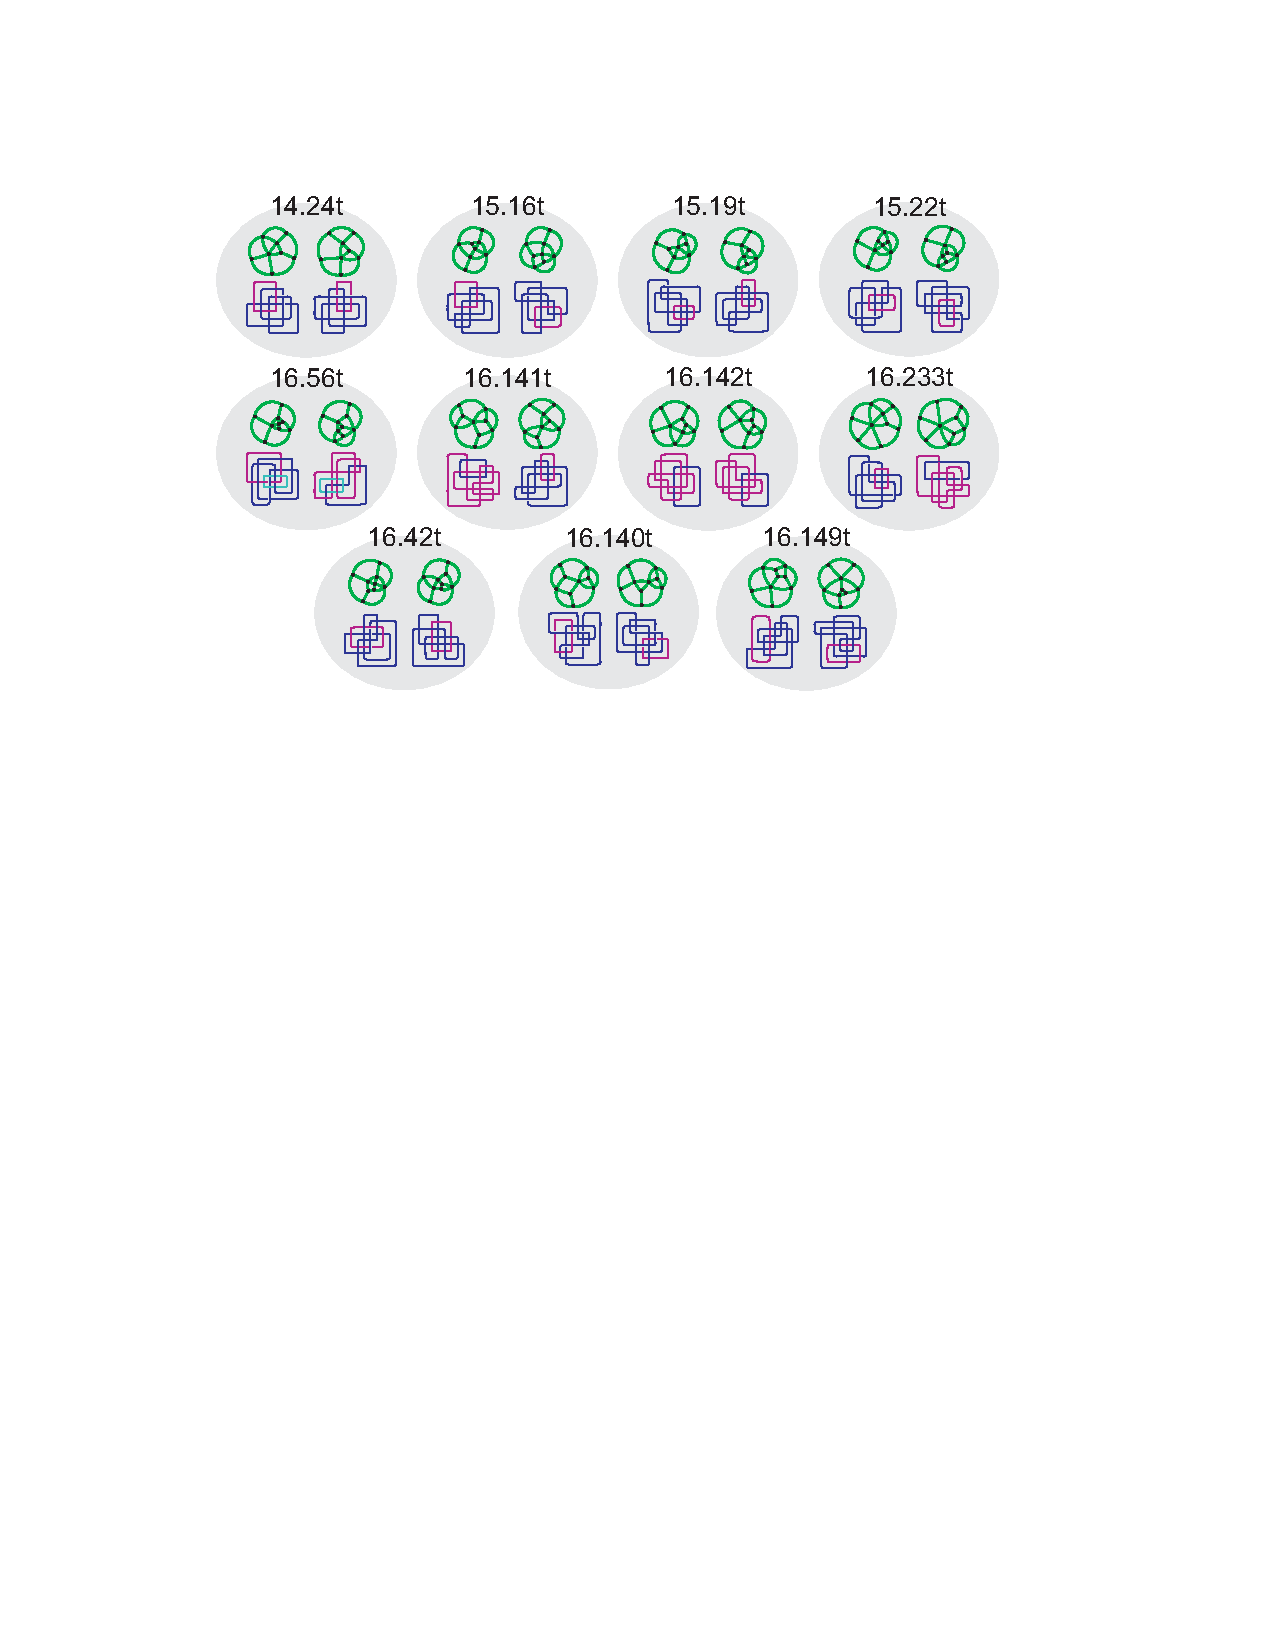
\includegraphics{fig/doubts3ConnectedIsolated.pdf}
\end{center}

\newcount\ii \newcount\jj   % declare integer variable
\def\producePagesThree#1#2{
\ii=#1                      % initialize ii
\jj=#2                      % initialize jj
\advance\jj by 1            % increment jj
\loop   % loop
   \ifnum\ii<\jj
{
   %\vspace{-1cm}
   %\thispagestyle{empty}
   % \setlength{\hoffset}{0cm}
   % \setlength{\textwidth}{\paperwidth-2cm}
   \hspace{-1.8cm}
   \enlargethispage{5cm}
   {\centering
   \includegraphics[width=18cm]{fig/con3catalog\ifnum\ii<100 0\fi\ifnum\ii<10 0\fi\number\ii.pdf}
   }
   \newpage}
      \advance\ii by 1
   \repeat
}

\newpage

\setlength{\topmargin}{-1.2cm}
%\setlength{\textwidth}{\paperwidth-2in}
%\setlength{\headheight}{1cm}
%\setlength{\headsep}{-3cm}
%\setlength{\footskip}{0.1cm}
%\setlength{\textheight}{\paperheight-\headheight-\headsep-\footskip-2in}
%\setlength{\oddsidemargin}{0mm}
%\setlength{\evensidemargin}{0mm}
%\setlength{\marginparwidth}{0mm}
%\setlength{\marginparsep}{0mm}
%\setlength{\textwidth}{\paperwidth-2in}

\producePagesThree{1}{39} 

%\newlength{\topmarginOne}
%\setlength{\topmarginOne}{\topmargin}
%\setlength{\topmargin}{\topmarginOne}
